
       \newpage
\chapter{DESIGN AND FABRICATION}


  

\begin{center}
    \section{Block Diagram}
\end{center}
\begin{figure}[H]
	\centering
	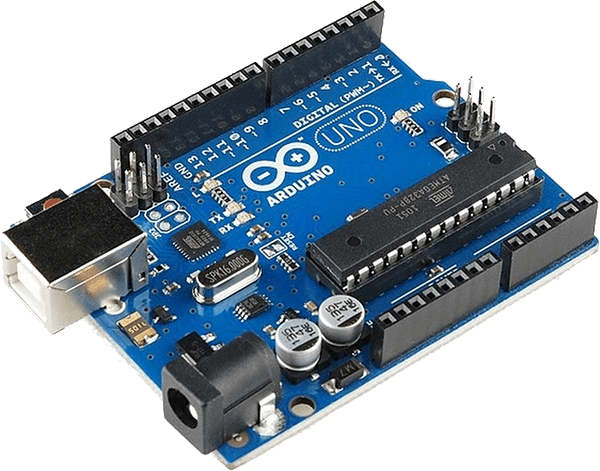
\includegraphics[width=10.75cm,height=8.44cm]{./images/image2.png}
        \caption{Arduino Uno R3}
	\end{figure}
\begin{center}
    [Replace the image with your Block Diagram]
\end{center}
   
        \newpage
  \begin{center}
      \section{Circuit Diagram}
  \end{center}
  \begin{figure}[H]
	\centering
	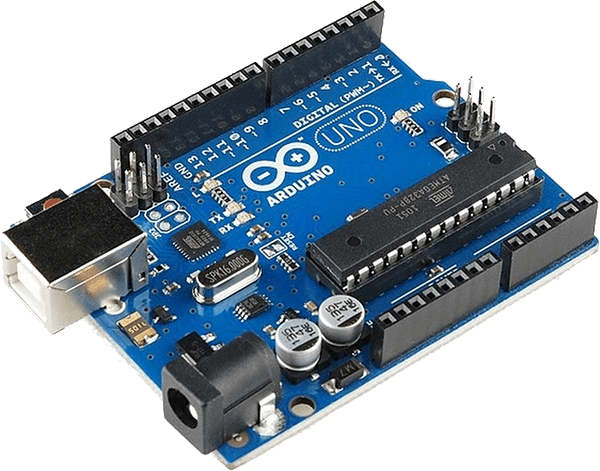
\includegraphics[width=10.75cm,height=8.44cm]{./images/image2.png}
        \caption{Arduino Uno R3}
	\end{figure}
 \begin{center}
     [Replace the image with your Circuit Diagram]
 \end{center}

 

\newpage
\begin{center}
    \section{Experimental Result}
\end{center}
Lorem Ipsum is simply dummy text of the printing and typesetting industry. Lorem Ipsum has been the industry's standard dummy text ever since the 1500s, when an unknown printer took a galley of type and scrambled it to make a type specimen book. It has survived not only five centuries, but also the leap into electronic typesetting, remaining essentially unchanged. It was popularised in the 1960s with the release of Letraset sheets containing Lorem Ipsum passages, and more recently with desktop publishing software like Aldus PageMaker including versions of Lorem Ipsum.
	\vspace{3\baselineskip}
    \begin{center}
        \Large Write here with your requirements.
    \end{center}
	\vspace{3\baselineskip}



\newpage
\begin{center}
    \section{Project Images}
\end{center}
\vspace{1\baselineskip}
	\begin{figure}[H]
	\centering
	\begin{subfigure}[b]{0.46\textwidth}
	\centering
	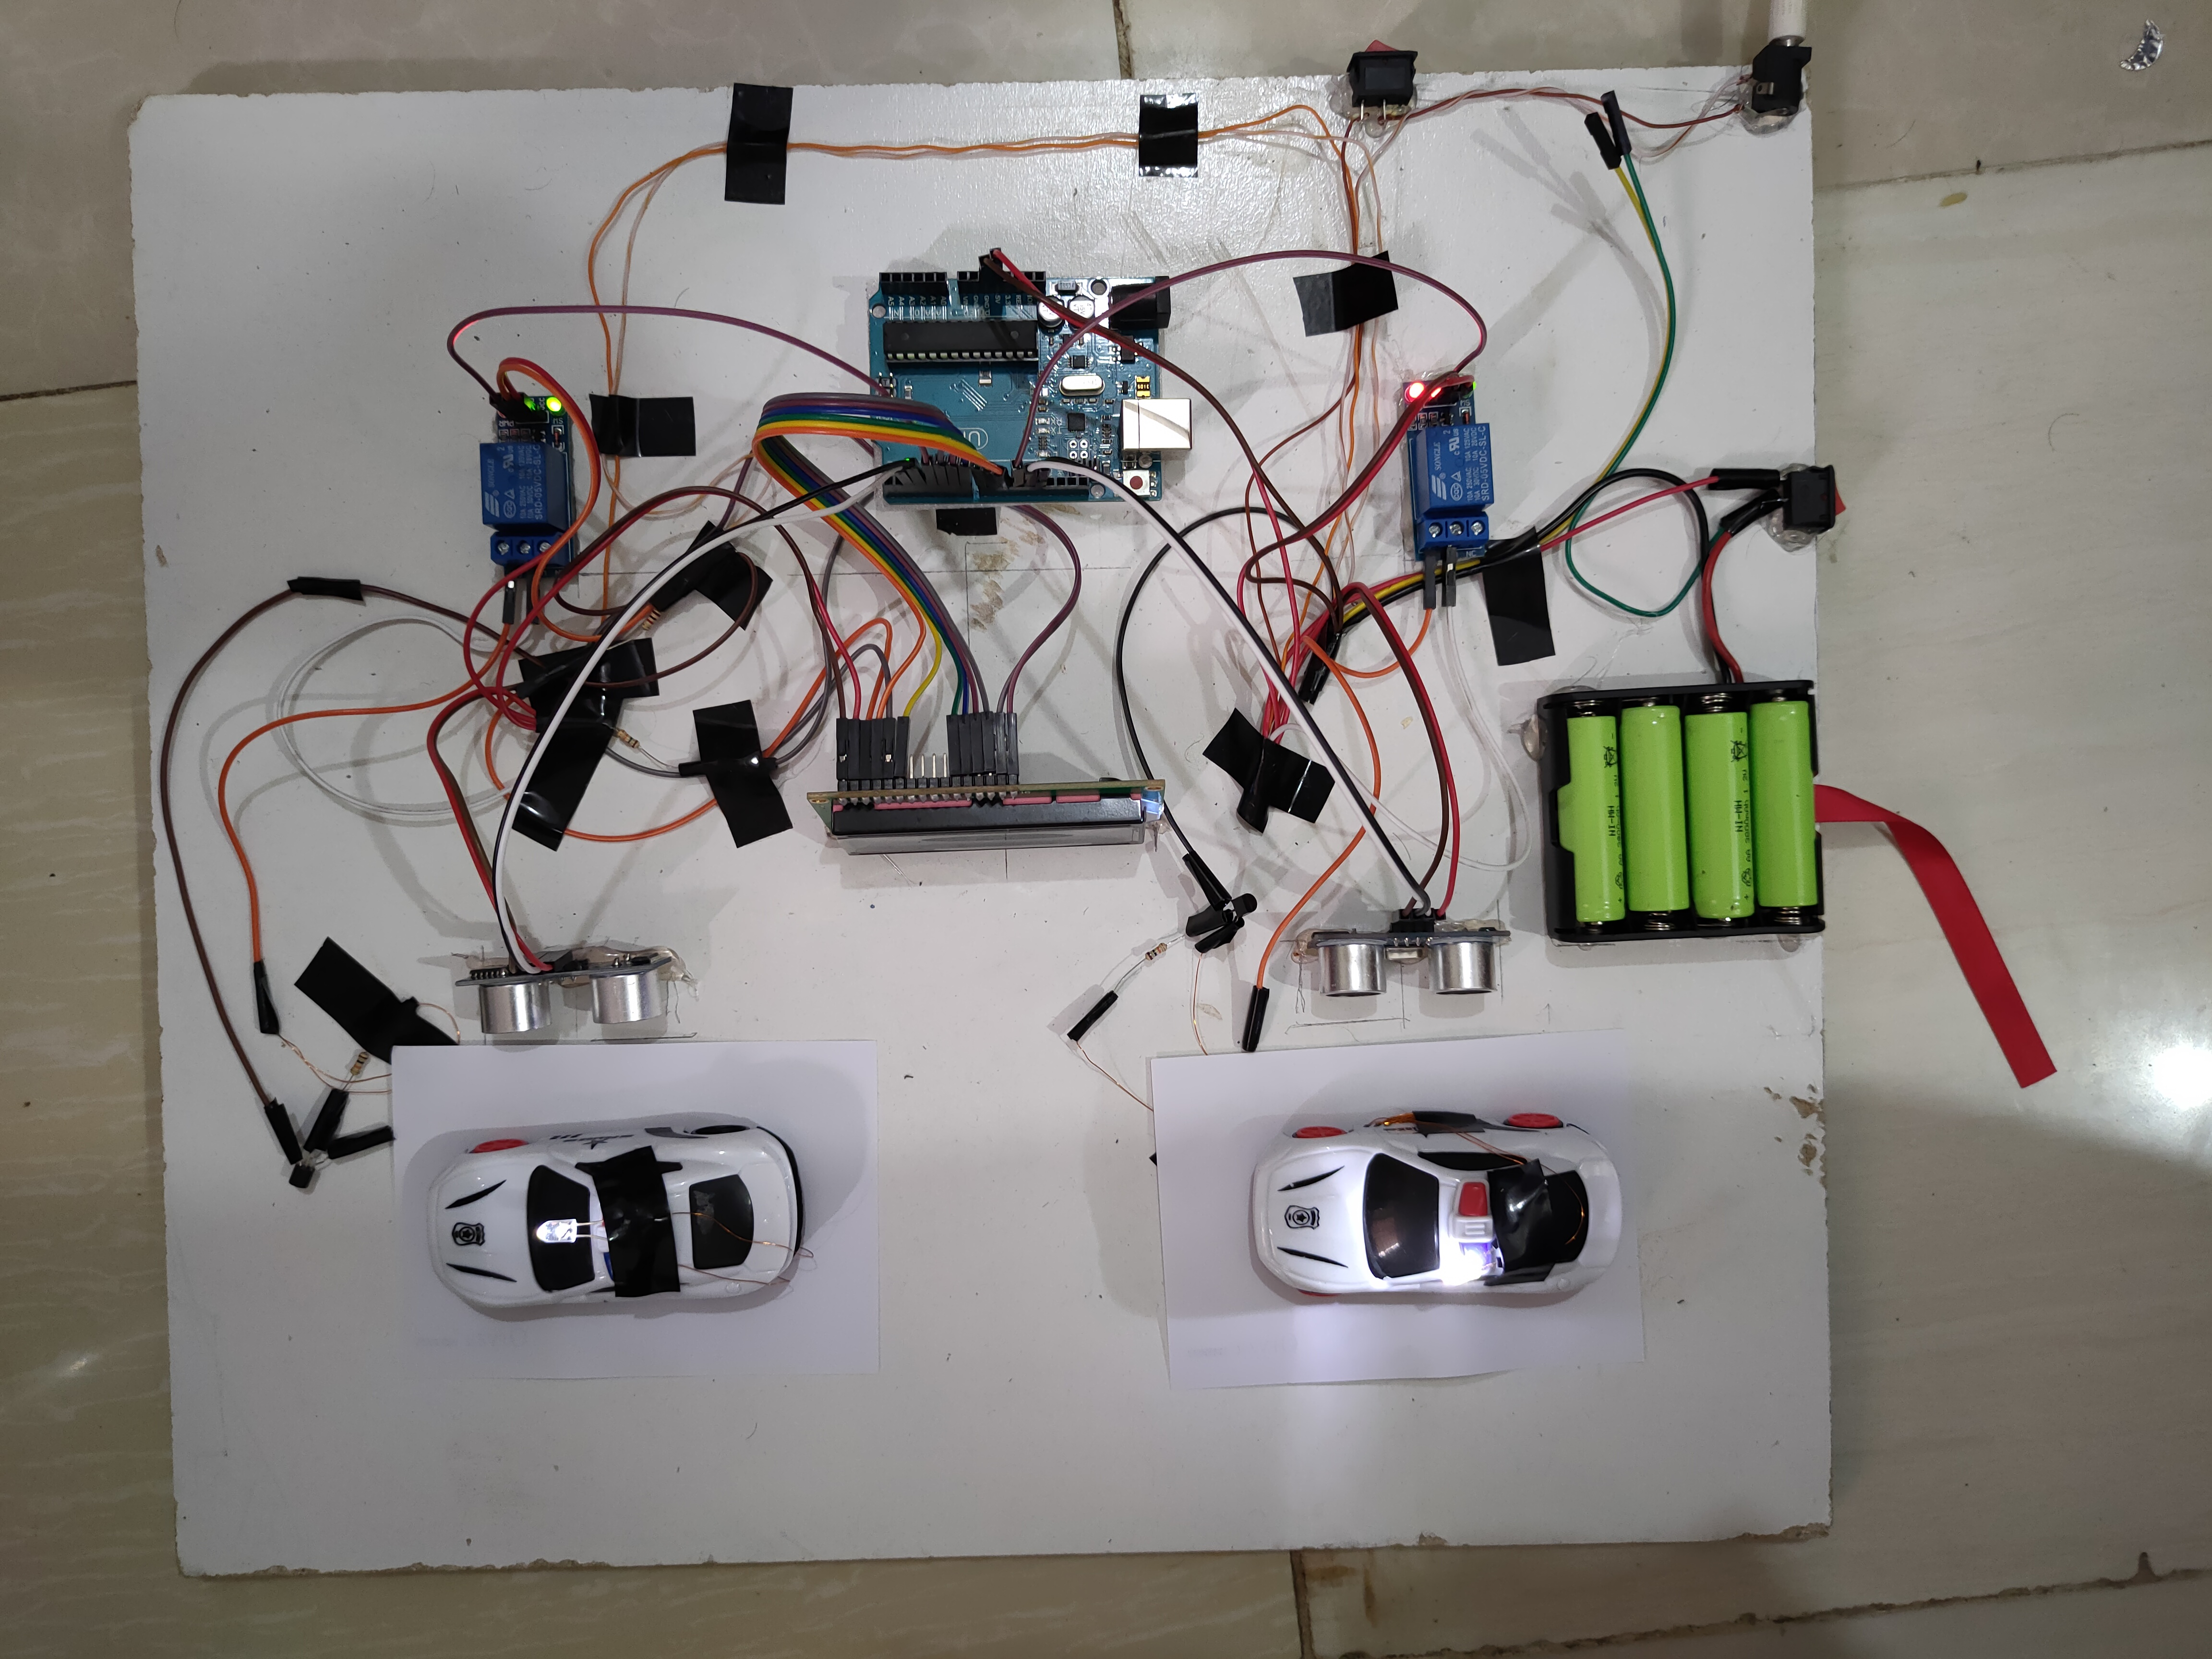
\includegraphics[width=\textwidth]{./figures/project_img1.jpg}
    \caption{Top View of the project}

	\end{subfigure}
	\hfill
	\begin{subfigure}[b]{0.46\textwidth}
	\centering
	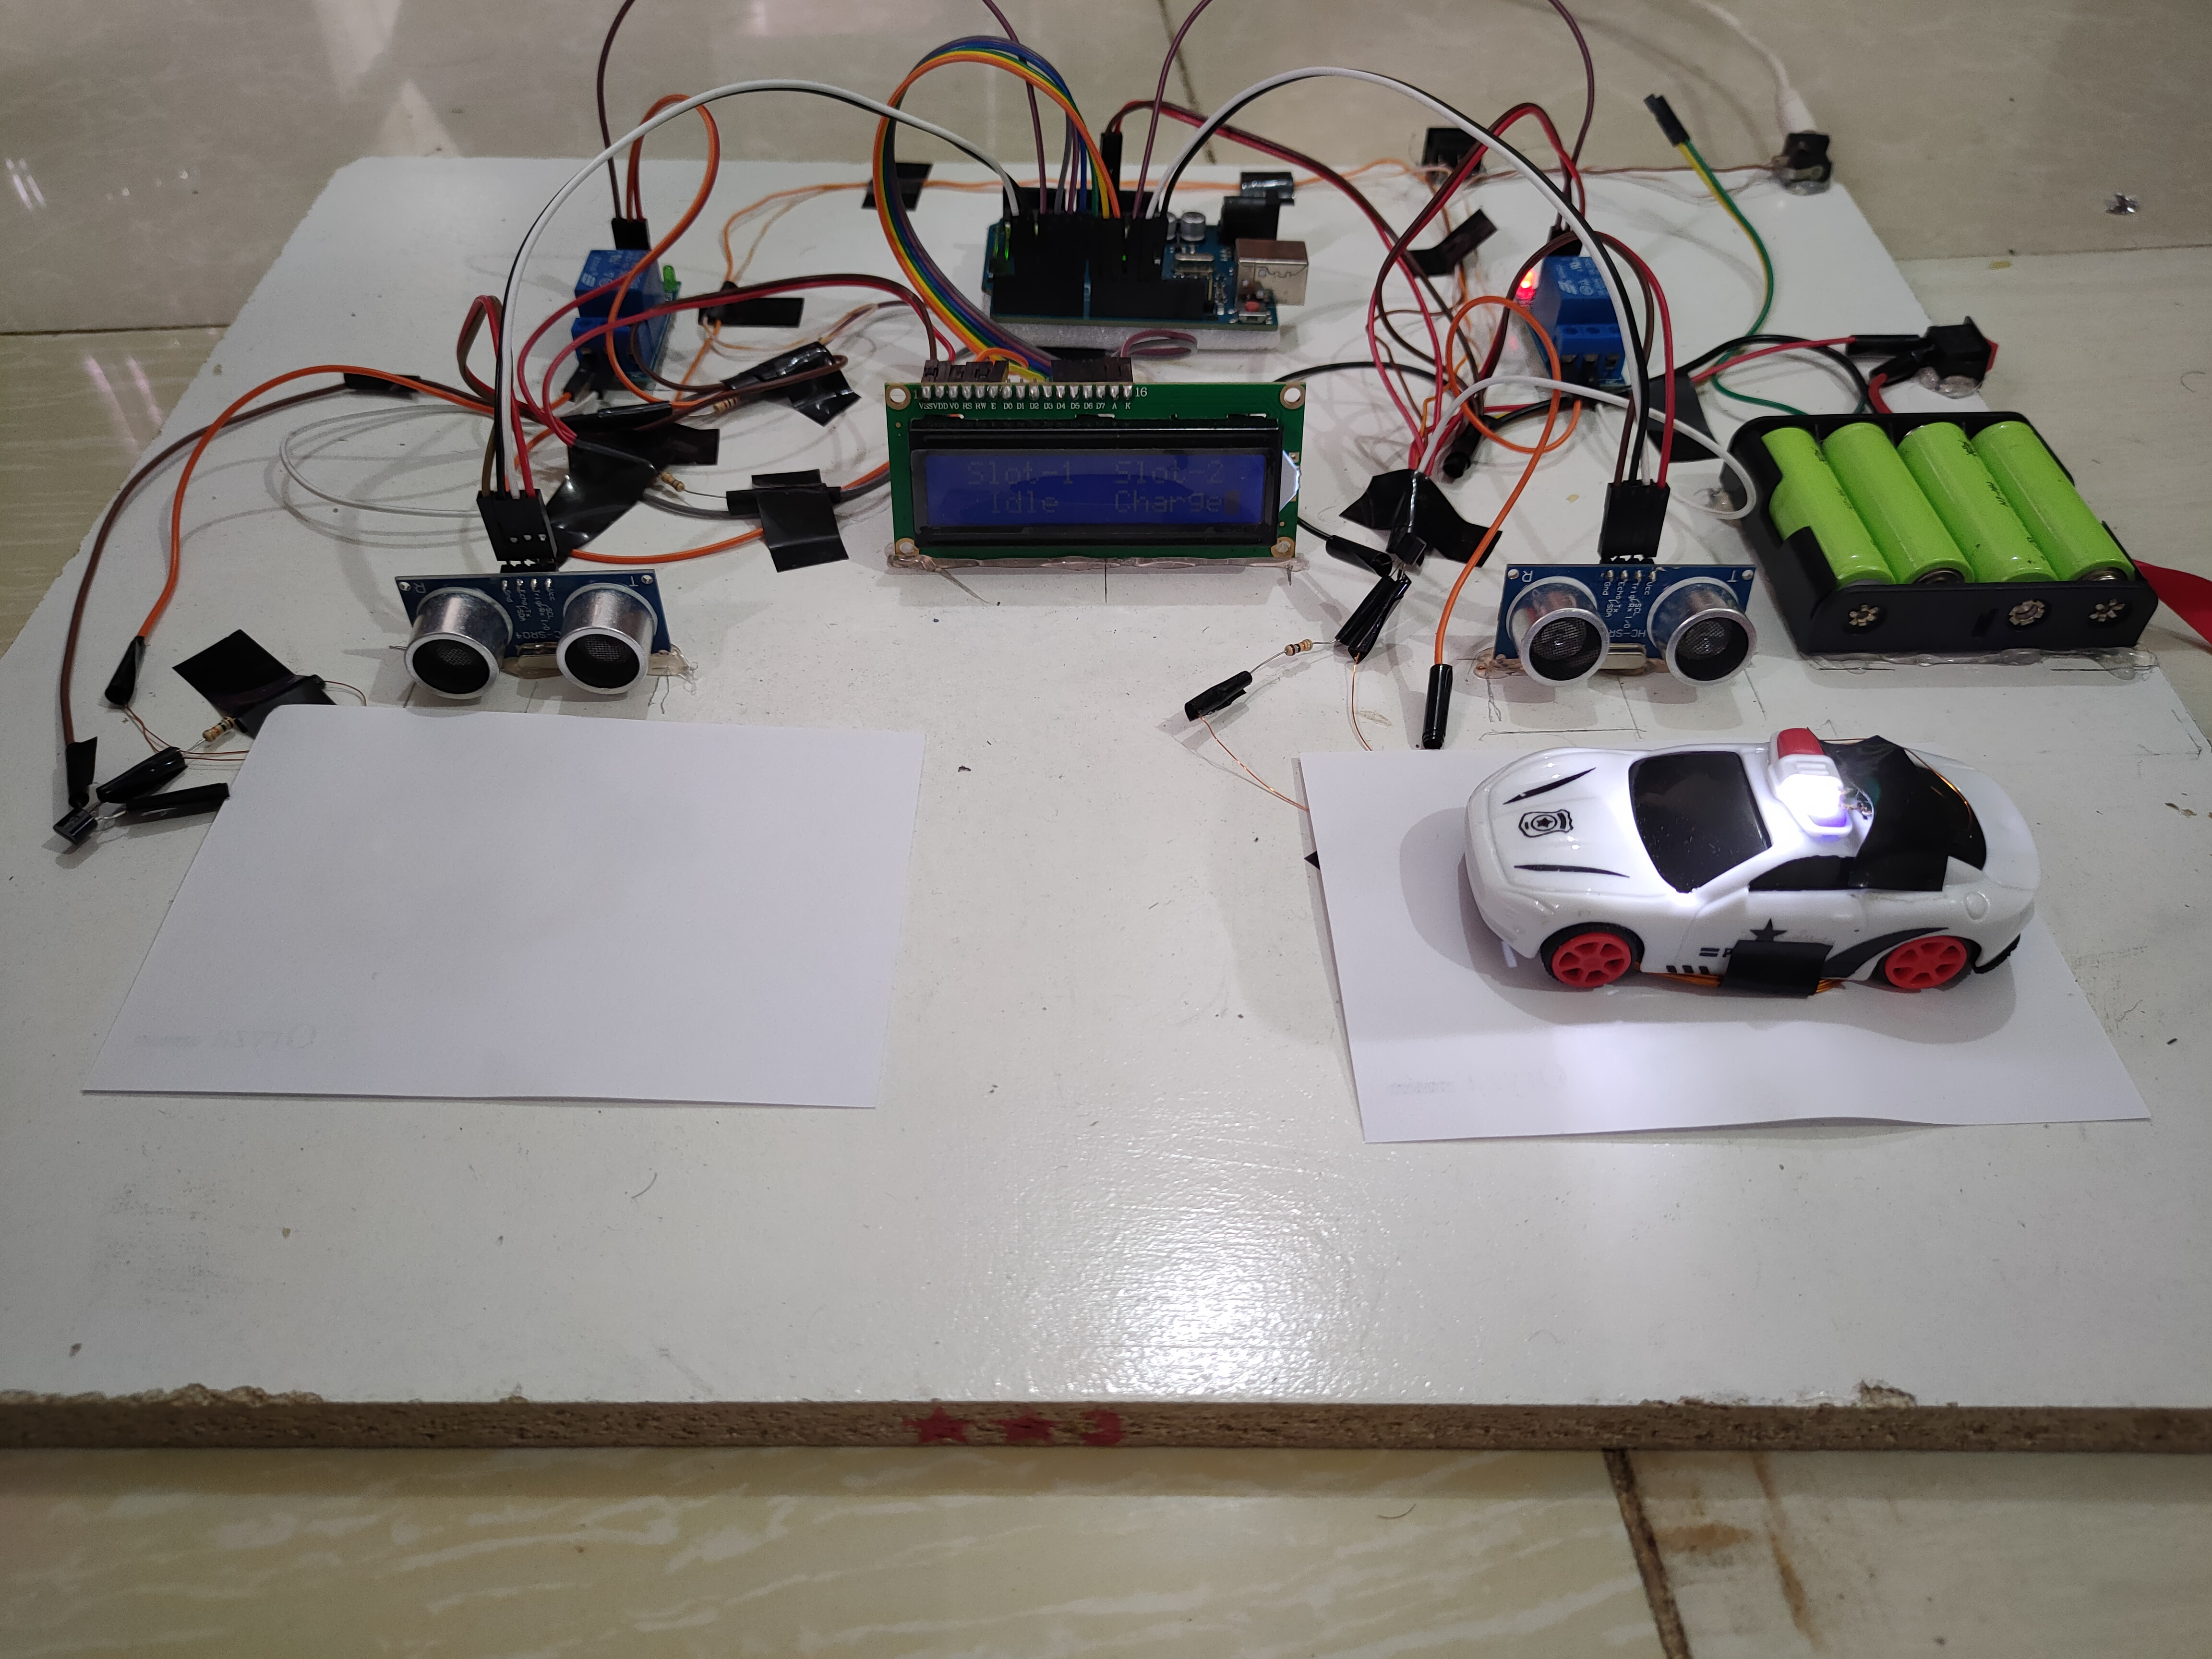
\includegraphics[width=\textwidth]
{./figures/project_img2.jpg}
\caption{Front View of the project}

	\end{subfigure}
	\end{figure}

\vspace{1\baselineskip}








\newpage
